\documentclass[a4paper,12pt,obeyspaces,spaces,hyphens]{article}

\def \trainingtype{onsite}
\def \agendalanguage{english}

\input{agenda/embedded-linux.inc}

\usepackage{agenda}

\begin{document}

\feshowtitle

\feshowinfo

\feagendatwocolumn
{Hardware platform for practical labs, option \#1}
{
  One of these Discovery Kits from STMicroelectronics: {\bf
  STM32MP157A-DK1}, {\bf STM32MP157D-DK1}, {\bf STM32MP157C-DK2} or
  {\bf STM32MP157F-DK2}
  \begin{itemize}
  \item STM32MP157, dual Cortex-A7 processor from STMicroelectronics
  \item USB powered
  \item 512 MB DDR3L RAM
  \item Gigabit Ethernet port
  \item 4 USB 2.0 host ports
  \item 1 USB-C OTG port
  \item 1 Micro SD slot
  \item On-board ST-LINK/V2-1 debugger
  \item Arduino compatible headers
  \item Audio codec, buttons, LEDs
  \item LCD touchscreen (DK2 kits only)
  \end{itemize}
}
{}
{
  \begin{center}
    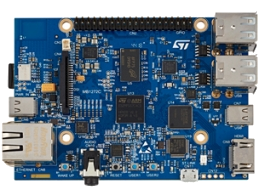
\includegraphics[width=5cm]{../slides/discovery-board-dk1/discovery-board-dk1.png}
  \end{center}
}

\feagendatwocolumn
{Hardware platform for practical labs, option \#2}
{
  {\bf BeagleBone Black} or {\bf BeagleBone Black Wireless} board
  \begin{itemize}
  \item An ARM AM335x (single Cortex-A8) processor from Texas
    Instruments
  \item USB powered
  \item 512 MB of RAM
  \item 2 or 4 GB of on-board eMMC storage
  \item USB host and device
  \item HDMI output
  \item 2 x 46 pins headers, to access UARTs, SPI buses, I2C buses
    and more.
  \item Ethernet or WiFi
  \end{itemize}
}
{}
{
  \begin{center}
    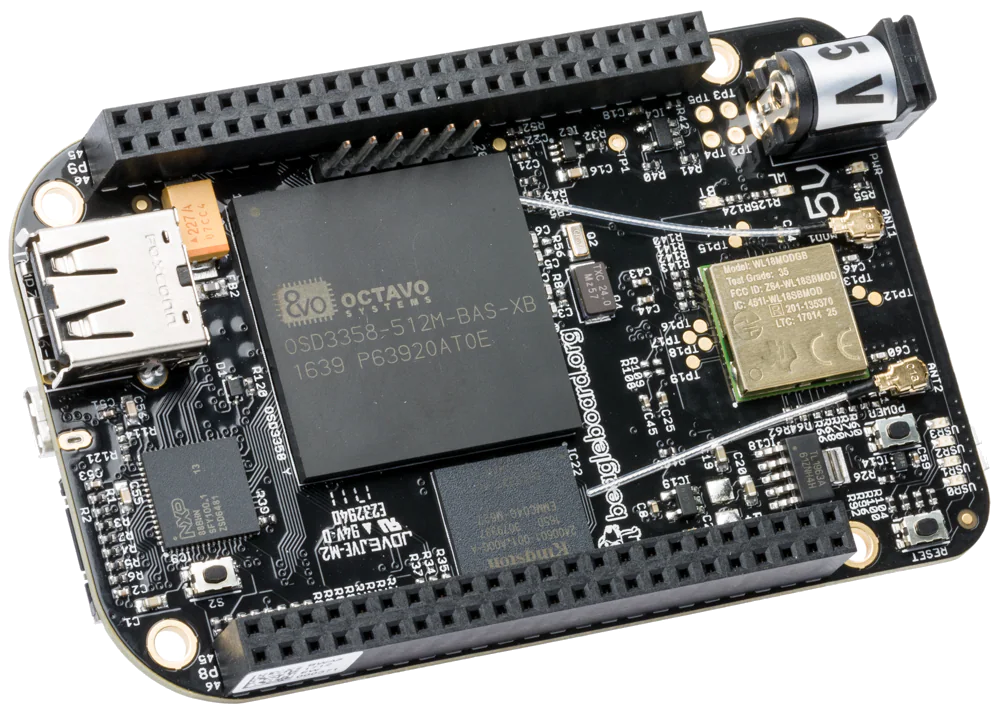
\includegraphics[width=5cm]{../slides/beagleboneblack-board/beagleboneblack.png}
  \end{center}
}

\section{Day 1 - Morning}

\feagendaonecolumn
{Lecture - Introduction to embedded Linux}
{
  \begin{itemize}
  \item Advantages of Linux versus traditional embedded operating
    systems.
  \item Typical hardware platforms used to run embedded Linux systems.
  \item Overall architecture of embedded Linux systems: overview of
    the major software components.
  \item Development environment for Embedded Linux development.
  \end{itemize}
}

\feagendatwocolumn
{Lecture - Cross-compiling toolchain and C library}
{
  \begin{itemize}
  \item What's inside a cross-compiling toolchain
  \item Choosing the target C library
  \item What's inside the C library
  \item Ready to use cross-compiling toolchains
  \item Building a cross-compiling toolchain with automated tools.
  \end{itemize}
}
{Lab - Cross compiling toolchain}
{
  \begin{itemize}
  \item Getting and configuring Crosstool-NG
  \item Executing it to build a custom cross-compilation toolchain
  \item Exploring the contents of the toolchain
  \end{itemize}
}

\section{Day 1 - Afternoon}

\feagendatwocolumn
{Lecture - Boot process, firmware, bootloaders}
{
  \begin{itemize}
  \item Booting process of embedded platforms, focus on the {\em x86}
    and {\em ARM} architectures
  \item Boot process and bootloaders on {\em x86} platforms (legacy
    and UEFI)
  \item Boot process on ARM platforms: ROM code, bootloaders, {\em ARM
      Trusted Firmware}
  \item Focus on U-Boot: configuration, installation, and usage.
  \item U-Boot commands, U-Boot environment, U-Boot scripts, U-Boot
    generic distro boot mechanism
  \end{itemize}
}
{Lab - Bootloader and U-boot}
{
  \begin{itemize}
  \item Set up serial communication with the board.
  \item Configure, compile and install U-Boot for the target hardware.
  \item Only on STM32MP1: configure, compile and install Trusted Firmare-A
  \item Become familiar with U-Boot environment and commands.
  \item Set up TFTP communication with the board. Use TFTP U-Boot
    commands.
  \end{itemize}

  \vspace{0.5cm}
  {\em Using the embedded hardware platform.}
}

\section{Day 2 - Morning}

\feagendatwocolumn
{Lecture - Linux kernel}
{
  \begin{itemize}
  \item Role and general architecture of the Linux kernel
  \item Separation between kernel and user-space, and interfaces
    between user-space and the Linux kernel
  \item Understanding Linux kernel versions: chosing between
    vendor-provided kernel and upstream kernel, {\em Long Term
      Support} versions
  \item Getting the Linux kernel source code
  \end{itemize}
}
{Lab - Fetching Linux kernel sources}
{
  \begin{itemize}
  \item Clone the mainline Linux tree
  \item Accessing stable releases
  \end{itemize}
}

\feagendatwocolumn
{Lecture - Configuring, compiling and booting the Linux kernel}
{
  \begin{itemize}
  \item Configuring the Linux kernel: ready-made configuration files,
    configuration interfaces
  \item Concept of {\em Device Tree}
  \item Cross-compiling the Linux kernel
  \item Study of the generated files and their role
  \item Installing and booting the Linux kernel
  \item The Linux kernel command line
  \end{itemize}
}
{Lab - Kernel cross-compiling and booting}
{
  \begin{itemize}
  \item Configuring the Linux kernel and cross-compiling it for the
    embedded hardware platform.
  \item Downloading your kernel on the board through U-boot's TFTP
    client.
  \item Booting your kernel.
  \item Automating the kernel boot process with U-Boot scripts.
  \end{itemize}

  \vspace{0.5cm}
  {\em Using the embedded hardware platform}
}

\section{Day 2 - Afternoon}

\feagendatwocolumn
{Lecture – Root filesystem in Linux}
{
  \begin{itemize}
  \item Filesystems in Linux.
  \item Role and organization of the root filesystem.
  \item Location of the root filesystem: on storage, in memory,
        from the network.
  \item Device files, virtual filesystems.
  \item Contents of a typical root filesystem.
  \end{itemize}
}
{Lecture - BusyBox}
{
  \begin{itemize}
  \item Detailed overview. Detailed features.
  \item Configuration, compiling and deploying.
  \end{itemize}
}

\feagendaonecolumn
{Lab – Tiny root filesystem built from scratch with BusyBox}
{
  \begin{itemize}
  \item Setting up a kernel to boot your system on a workstation
    directory exported by NFS
  \item Passing kernel command line parameters to boot on NFS
  \item Creating the full root filesystem from scratch.
    Populating it with BusyBox based utilities.
  \item System startup using BusyBox \code{init}
  \item Using the BusyBox HTTP server.
  \item Controlling the target from a web browser on the PC host.
  \item Setting up shared libraries on the target and compiling
    a sample executable.
  \end{itemize}

  \vspace{0.5cm}
  {\em Using the embedded hardware platform}
}

\section{Day 3 - Morning}

\feagendatwocolumn
{Lecture - Accessing hardware devices}
{
  \begin{itemize}
  \item How to access hardware on popular busses: USB, SPI, I2C, PCI
  \item Usage of kernel drivers and direct user-space access
  \item The {\em Device Tree} syntax, and how to use it to describe
    additional devices and pin-muxing
  \item Finding Linux kernel drivers for specific hardware devices
  \item Using kernel modules
  \item Hardware access using \code{/dev} and \code{/sys}
  \item User-space interfaces for the most common hardware devices:
    storage, network, GPIO, LEDs, audio, graphics, video
  \end{itemize}
}
{Lab - Accessing hardware devices}
{
  \begin{itemize}
  \item Exploring the contents of \code{/dev} and \code{/sys} and the
    devices available on the embedded hardware platform.
  \item Using GPIOs and LEDs.
  \item Modifying the Device Tree to control pin multiplexing and
        to declare an I2C-connected joystick.
  \item Adding support for a USB audio card using Linux kernel modules
  \item Adding support for the I2C-connected joystick through
        an out-of-tree module.
  \end{itemize}

  \vspace{0.5cm}
  {\em Using the embedded hardware platform}
}

\section{Day 3 - Afternoon}

\feagendatwocolumn
{Lecture - Block filesystems}
{
  \begin{itemize}
  \item Accessing and partitioning block devices.
  \item Filesystems for block devices.
  \item Usefulness of journaled filesystems.
  \item Read-only block filesystems.
  \item RAM filesystems.
  \item How to create each of these filesystems.
  \item Suggestions for embedded systems.
  \end{itemize}
}
{Lab - Block filesystems}
{
  \begin{itemize}
  \item Creating partitions on your SD card
  \item Booting a system with a mix of filesystems: {\em SquashFS} for
    the root filesystem, {\em ext4} for system data, and {\em
      tmpfs} for temporary system files.
  \end{itemize}

  \vspace{0.5cm}
  {\em Using the embedded hardware platform}
}

\feagendaonecolumn
{Lecture - Flash filesystems}
{
  \begin{itemize}
  \item The Memory Technology Devices (MTD) filesystem.
  \item Filesystems for MTD storage: JFFS2, Yaffs2, UBIFS.
  \item Kernel configuration options
  \item MTD storage partitions.
  \item Focus on today's best solution, UBI and UBIFS:
	preparing, flashing and using UBI images.
  \end{itemize}

  \vspace{0.5cm}

  {\em Note: as the embedded hardware platform used for the labs does
    not have any flash-based storage, this lecture will not be
    illustrated with a corresponding practical lab.}
}

\section{Day 4 - Morning}

\feagendatwocolumn
{Lecture – Cross-compiling user-space libraries and applications}
{
  \begin{itemize}
  \item Configuring, cross-compiling and installing applications and
    libraries.
  \item Concept of build system, and overview of a few common build
    systems used by open-source projects: Makefile, {\em autotools},
    {\em CMake}, {\em meson}
  \item Overview of the common issues encountered when
    cross-compiling.
  \end{itemize}
}
{Lab – Cross-compiling applications and libraries}
{
  \begin{itemize}
  \item Manual cross-compilation of several open-source libraries and
    applications for an embedded platform.
  \item Learning about common pitfalls and issues, and their
    solutions.
  \item This includes compiling {\em alsa-utils} package,
    and using its \code{speaker-test} program to test that
    audio works on the target.
  \end{itemize}

  \vspace{0.5cm}
  {\em Using the embedded hardware platform}
}

\section{Day 4 - Afternoon}

\feagendatwocolumn
{Lecture - Embedded system building tools}
{
  \begin{itemize}
  \item Approaches for building embedded Linux systems: build systems
    and binary distributions
  \item Principle of {\em build systems}, overview of Yocto
    Project/OpenEmbedded and Buildroot.
  \item Principle of {\em binary distributions} and useful tools,
    focus on Debian/Ubuntu
  \item Specialized software frameworks/distributions: Tizen, AGL,
    Android
  \end{itemize}
}
{Lab - System build with Buildroot}
{
  \begin{itemize}
  \item Using Buildroot to rebuild the same basic system
        plus a sound playing server ({\em MPD}) and a
        client to control it ({\em mpc}).
  \item Driving music playback, directly from the target,
        and then remotely through an MPD client on the
	host machine.
  \item Analyzing dependencies between packages.
  \end{itemize}

  \vspace{0.5cm}
  {\em Using the embedded hardware platform}
}

\feagendaonecolumn
{Lecture - Open source licenses and compliance}
{
  \begin{itemize}
  \item Presentation of the most important open-source licenses: GPL,
    LGPL, MIT, BSD, Apache, etc.
  \item Concept of {\em copyleft} licenses
  \item Differences between (L)GPL version 2 and 3
  \item Compliance with open-source licenses: best practices
  \end{itemize}
}

\section{Day 5 - Morning}

\feagendatwocolumn
{Lecture - Overview of major embedded Linux software stacks}
{
  \begin{itemize}
  \item \code{systemd} as an {\em init} system
  \item Hardware management with {\em udev}
  \item Inter-process communication with {\em D-Bus}
  \item The connectivity software stack: Ethernet, WiFi, modems,
    Bluetooth
  \item The graphics software stack: DRM/KMS, X.org, Wayland, Qt, Gtk,
    OpenGL
  \item The multimedia software stack: Video4Linux, GStreamer,
    Pulseaudio, Pipewire
  \end{itemize}
}
{Lab - Integration of additional software stacks}
{
  \begin{itemize}
  \item Integration of {\em systemd} as an init system
  \item Use {\em udev} built in {\em systemd} for automatic module
    loading
  \end{itemize}

  \vspace{0.5cm}
  {\em Using the embedded hardware platform}
}

\section{Day 5 - Afternoon}

\feagendatwocolumn
{Lecture - Application development and debugging}
{
  \begin{itemize}
  \item Programming languages and libraries available.
  \item Build system for your application, an overview of {\em CMake}
    and {\em meson}
  \item The {\em gdb} debugger: remote debugging with {\em gdbserver},
    post-mortem debugging with \code{core} files
  \item Performance analysis, tracing and profiling tools, memory
    checkers: \code{strace}, \code{ltrace}, \code{perf},
    \code{valgrind}
  \end{itemize}
}
{Lab – Application development and debugging}
{
  \begin{itemize}
  \item Creating an application that uses an I2C-connected joystick to
    control an audio player.
  \item Setting up an IDE to develop and remotely debug an
    application.
  \item Using {\em strace}, {\em ltrace}, {\em gdbserver} and {\em
      perf} to debug/investigate buggy applications on the embedded
    board.
  \end{itemize}

  \vspace{0.5cm}
  {\em Using the embedded hardware platform}
}

\feagendaonecolumn
{Lecture - Useful resources}
{
  \begin{itemize}
  \item Books about embedded Linux and system programming
  \item Useful online resources
  \item International conferences
  \end{itemize}
}

\end{document}
